\setcounter{chapter}{3}

\chapter{Distributed Decision Making for Dynamic Formation of Web Services Communities}\label{cha:PCTLKC}


\section{Introduction}

Over the past years, online services have become an important part of many scalable business applications. The increasing reliance on online service providers has significantly influenced the way web services are engineered. Given the dynamic and unpredictable nature of the Internet, delivering high quality services is still a critical and challenging issue. One practical solution towards delivering such quality services is utilizing intelligent decision making agents. These agents aim at maximizing their gain by exploring the best ways to provide services that satisfy end users \cite{Zeng:2003:QDW:775152.775211, 10.1109/ARES.2008.7, Demirkan2013412, journals/tsc/ZhengZYB13, Josang:2007:STR:1225318.1225716}. However, agent-based web services are functionally limited in the sense that they cannot handle a large number of requests at the same time without compromising the quality of service provided. Recent developments have attempted to shift web services from simple models, consisting of individual components, to models made up of autonomous and group-based components that share common goals. In group-based models, interaction, composition, and cooperation are the key challenges that directly impact the group's overall performance in achieving common goals \cite{ICWS2011-1, SCC2011-1, journals/mags/BaldoniBM10, journals/jcss/CasadoYT13}. To that end, we see the emergence of web service \emph{communities}, which consist of grouping services with similar functionalities but distinct nonfunctional properties \cite{Zeng:2003:QDW:775152.775211, 10.1109/ARES.2008.7, Paik:2005:TSS:2229263.2230038, Medjahed05adynamic}. A community of web services runs continuous performance assessment functions that regulate web services' interactions and manage their composition and cooperation.

Web Service communities have the advantages of facilitating web service discovery and providing better quality of service compared to individual services. Communities act as abstract web services, communicating with external entities via the same standard protocols that a normal web service employs. The difference is that communities regulate the service process via sophisticated internal communication protocols, thereby providing services based on the combined efforts of a number of web services. The downside to communities is the complexity of management involved in finding and inviting adequate individual services and managing the overall quality of the combined work of several services.
% because although they have similar functionality, they have different attitudes.
When interacting with a community of web services, users send their requests to the coordinator of the community, which plays the role of community representative or access point. The community coordinator is responsible of receiving tasks and delivering services. Moreover, as community representative, it verifies the credentials of new web services before accepting them into the community and kicks services that could harm the value of the community.

\textbf{Challenges and Problem Statement.} In recent work, communities of web services have been proposed in order to facilitate discovery of web services, improve the Quality of Service (QoS), and help individual services find better market share and opportunities \cite{Zeng:2003:QDW:775152.775211, 10.1109/ARES.2008.7, Paik:2005:TSS:2229263.2230038, Medjahed05adynamic}. However,  two important challenges are to be addressed: 1) choice of the best web services during community development from the community perspective; and 2) choice of the best community to join from the web service perspective. The advocated solutions  \cite{10.1109/ARES.2008.7, conf/webist/MaamarLBTS07, journals/soca/XuYLZB11, 10.1109/TSC.2012.12, managing-hela-jalel, DBLP:conf/IEEEscc/KhosravifarABT11, DBLP:conf/IEEEscc/LimTMB12} have attempted to address these challenges. However, those solutions have two main limits:
\begin{enumerate}
	\item The solutions consider the architecture of centralized management for communities where most of the decisions are made by the centralized coordinator. The problem is that in real world scenarios, decisions made by independent service providers are highly distributed.
	\item The solutions either propose complex algorithms \cite{10.1109/TSC.2012.12, DBLP:conf/IEEEscc/LimTMB12, journal-community-formation} to find the optimal strategy to follow, or oversimplify the problem by eliminating important parameters and using approximation techniques to make the algorithms tractable \cite{10.1109/TSC.2012.12}.
\end{enumerate}
These approximation methods sometimes negatively influence the outcome because simplifying the constraints may cause important aspects of the problem to be ignored. For instance, instead of calculating the gain distribution using the adequate, but complex shapely-value method, the authors is \cite{10.1109/TSC.2012.12} propose a simple egalitarian way of distributing gain, which completely ignores the gain generated from collaborative work of sub-communities. Other categories of related work, for instance \cite{10.1109/TSC.2012.12, DBLP:conf/IEEEscc/KhosravifarABT11, DBLP:journals/ijebr/MaamarSTBB09}, restrict the decision process within the community coordinator, so other members of the community are not effectively involved.
%And some other work which do not focus on rationality on web services or communities involved [refrences].
In \cite{journal-community-formation}, we proposed a cooperative game-theory-based model for aggregating web services in communities. A centralized decision maker in communities, based on a complete knowledge of available web service quality metrics and performance, has been used to form optimal and stable communities that maximize individual and group income. However, centrality and complete information are strong assumptions, which are not very compatible with real business scenarios.

\textbf{Contributions.} In this chapter, we introduce DDM, a Distributed Decision Making model for community formation that regulates web service agents’ decision making process in terms of cooperating and deciding which group to join and which service to invite for joining. Unlike existing work on community formation, our decision model is extracted from a data model in the form of information obtained from a large number of web services regarding their single and cooperative utilities as well as environmental parameters such as demand, service quality, etc. The generated decision tree improves agents' understanding of the environment and how to select actions that lead towards maximizing their utilities. The advantage of this approach is that the tree, which is initially created from the past data, reflects a comprehensive vision about agents' attitudes in terms of their action selection based on their past experiences. Moreover, the tree is getting continuously updated based on both new received feedback and the outcome of chosen actions. This continuous update makes the approach adapted to any change in the environment.
%The training model deploys a logistic regression algorithm to build a hypothesis function that can thoroughly address the aforementioned research problems.
The decision model provides web services with enough information which helps those services efficiently decide and predict the outcome of their different possible collaborations. This model works in a distributed manner in which services are self-sufficient in their decision making and do not rely on a centralized decision making process. Our findings show that communities of web services can efficiently find the appropriate web service to invite for cooperation as well as allowing a single web service to find the best communities to join. The proposed model can be seen as a recommneder system that suggests beneficial actions for both communities and single services. Communities can consider the decision model and analyze the characteristics of different individual web services and make prudent decisions when inviting a web service to join or accepting a join inquiry initiated from a web service. In general, DDM equips web services with efficient methods for foreseeing how their choices will impact both their short-term and long-term goals; therefore, opting for the best decision available.

To effectively generate the decision model for web services, we used a real dataset to extract web services' individual characteristics and used them to measure outcomes when these services cooperate with one another. The dataset has been extracted from real-world QoS evaluation results from 142 users on 4,532 Web services during 64 different time slots. Combining the available data based on each web service point of view on different time slots, we acquired 5 different unique features for those 4,532 web services. By engineering and extracting these features, we gathered functional and cooperative features for both individual web services and communities in different time slots. We were able to investigate the path a web service might take to achieve the best utility out of effective interactions with others. All the paths and outcomes are labeled to be utilized in the training model. Using cross validation sets, web services are able to compute the optimal hypothesis function (using logistic regression) that can be used to predict outcomes of cooperative work with other individual web services or communities. Our findings show that web services equipped with DDM have by far better outcomes than the ones that either do not cooperate or randomly find communities to join.

\section{Preliminaries and Challenging Issues}\label{s4:preliminaries}
%In this section, we first present the architecture of DDM. We explore the characteristics of intelligent service agents and the features we extract for training. To do this, we first discuss some preliminaries.
In this section, we discuss the preliminary concepts of communities of web services and introduce the challenges behind community formation.

\subsection{Web Services}\label{s:ws}

In the recent years, online services have become a standard part of daily life around the globe. Many modern applications rely on web services from different providers. For instance, many mobile and tablet applications that have limited storage and processing power are merely aggregating information from different online services. Examples are vast, including weather forecasting, ticket selling, shopping apps, local maps and location services.

The World Wide Web Consortium (W3C) defines web services as ``software systems designed to support interoperable machine-to-machine interaction over a network. It has an interface described in a machine-processable format (specifically WSDL). Other systems interact with the web service in a manner prescribed by its description using SOAP messages, typically conveyed using HTTP with XML serialization in conjunction with other Web-related standards''. When developers declare a new web service, it will be
discovered based on its description, which fully discloses its functionalities. Developers also have to declare a public interface and a readable documentation to help other developers when integrating different services \cite{w3cwsdl}. Nowadays, web API, standards that do not require XML-based web service protocols like SOAP and WSDL are also emerging. They are called RESTful (representational state transfer) services, which are moving towards simpler communication protocols.
%They are not restricted
%to XML formats, recently JSON, a human readable and simpler format
%is becoming popular among online service providers.

We are not going to delve into the engineering details of online web service implementation and its protocols in this thesis. We are interested in web services from a business model perspective. Service providers usually charge end users for services they provide. For example, Google has listed pricing and plans for a wide range of services they provide on their web service console page\footnote{$https://code.google.com/apis/console$}.

As in other proposals \cite{journals/mags/BaldoniBM10,10.1109/TSC.2012.12,DBLP:conf/IEEEscc/KhosravifarABT11}, in this paper, we abstract web services as rational agents\footnote{The term rational is used here in the sense that web services are utility maximizers.} that provide services to end users. They aim to maximize their individual income  by receiving enough requests from end users. In order to increase their revenues, web services seek for more tasks if they have the capacity and throughput to do so. Web services can join communities to enhance efficiency by collaborating with others, to have access to broad market share, and for the opportunity to receive a bigger task pool from end users.
Furthermore, the high reliance on web services has resulted in increased quality expectations from end users. Communities of web services can provide higher availability, performance, reliability, and recovery for end users.

\subsection{Web Service Communities}\label{s:wsc}

The community of web services is essentially a virtual group of web services having similar functionalities \cite{DBLP:journals/ijebr/MaamarSTBB09}. Communities aggregate web services and communicate with other entities such as UDDI registries and users, using identical protocols to those used by single web services. Web services join communities to increase utility by having a larger market share and task pool. The community coordinator is responsible for securing the community, managing membership requests from web services and distributing user tasks among the community members. The coordinator tries to attract quality web services to join and keep the community as stable and productive as possible to gain better reputation and user satisfaction, which increases the community's market share. How web services reside within communities and how communities of web services are engineered is described comprehensively in \cite{DBLP:journals/ijebr/MaamarSTBB09}.

\subsection{The Join Challenge}\label{s:tjc}
It has been showed in \cite{10.1109/ARES.2008.7,10.1109/TSC.2012.12,journal-community-formation} that web services can increase their overall utility by collaborating with other web services within communities. This collaboration provides them with better ways of sharing resources and having higher reputation, greater market share and wider visibility. Web services and communities come with different quality metrics, and the long-term outcome depends on these metrics.

The goal of all parties involved in the community is to maximize their long-term outcome while they are operating as part of the community. Web services need to be equipped with a selection strategy to choose from the different possible collaboration groups they can form as well as an estimation method for evaluating the long-term gain of joining different possible communities. Web services need to experiment with different possible collaborative groups in order to estimate their gain over time. However, with a high number of possible communities, it is not possible to test collaboration with random web services. Even if a linear approximate function for estimating utility based on community web services' parameters is adopted, the exponential \footnote{Bell number: $http://en.wikipedia.org/wiki/Bell\_number$} growth rate of the possible number of partitions of web services into communities would make any brute-force type algorithm for the best community selection strategy intractable and impractical in real-world application settings.

\subsection{Join Consequences}\label{s:jc}
It is worth mentioning that a \emph{join} event takes place as a result of interaction between two parties that are looking to expand their collaborations. All actions are chosen in an attempt to enhance the overall outcome. However, the selected action may result in decreasing the overall utility in the long run.
% long term.
This is the case when a single web service joins a community, but the complex process of task allocation eliminates the visibility of that service, which stays idle within the community. This makes the join action of that service a bad decision. The same event might be beneficial for the community, as it hosts a new web service that can engage in performing a new coming task. But overall, in this particular case, if the new web service stays idle for a long period of time, neither side will benefit from collaborating with the other and the join event will result in negative consequences for at least one side's utility.

The more common scenario is when both parties benefit from the joining of a web service to a community. This joining action is then rational as both the web service and community enhance their utilities. However, the community may not be the best choice for the web service. In other words, the web service could have joined a better community if it had enough and accurate knowledge about the surrounding environment. Since the community does enhance its utility, the web service could stay with that community, which results in a non-optimal increase in web service's utility. In the following section, the proposed model provides solutions that effectively address the aforementioned challenges.

\section{The Model Components}\label{s:themodelcomponents}

In this section, we discuss the parameters that we use in the rest of the chapter. Then, we present the task distribution and revenue model of our distributed web services communities.

\subsection{Internal Features}\label{s:if}

With a group of web services having identical or similar functionalities, QoS metrics provide nonfunctional characteristics for optimal candidate selection. Web services quality metrics have been studied and analyzed in various proposals, for instance in in \cite{Ardagna:2007:ASC:1263152.1263531,Menasce:2002:QIW:613357.613758,10.1109/ISSRE.2011.17}. In this chapter, we adopt the most representative QoS properties of those services that highly influence their utility.
%We refer to a typical web service as ws_{i}.

Let $C = \{ws_1,ws_2,..., ws_n\}$ be a community with $n$ web services. We define the following features for the group of web services based on their functional parameters:

\begin{itemize}

  \item \emph{Throughput} is the rate at which a service can process requests. QoS measures can include the maximum throughput or a function that describes how throughput varies with load intensity. Throughput is a positive real number. For a given community $C$, the expected throughput value $(Th_{C})$ can be estimated as the summation of throughput of all the service members $Th_{w}~ (w \in C)$:
	
	\begin{equation}
		 Th_{C} = \sum_{w \in C}{(Th_{w})}
	\end{equation}
	
	\item \emph{Availability} is the percentage of time that a service is operating. It is computed as
the probability that the service operation is accessible. Availability of a web service $A_w$ is a real number in the range $[0, 1]$. For a community $C$, the expected availability $(A_{C})$ considering the members operate in parallel (independently from each other) can be estimated as:
	
	\begin{equation}
		A_{C} = 1-\prod_{w \in C}{(1-A_{w})}
	\end{equation}
	
	\item \emph{Execution Time} is the time a service takes to respond to various types of requests.
	%is the expected delay between the time instant when a request is sent and the time when the result is obtained.
	Execution time is usually measured in milliseconds and can be affected by load intensity, which can be measured in terms of arrival rates (such as requests per second) or number of concurrent requests. This internal feature is a positive integer. For a typical community $C$, the expected execution time $Et_{C}$ can be estimated as the execution time of the bottleneck service which is the service with the slowest execution time $Et_{w}$:
	
	\begin{equation}
		Et_{C} = max_{w \in C}{(Et_{w})}
	\end{equation}
	
	%\item \emph{Data Quality} The ability of a data collection to meet user requirements , defined as the proximity of a value v returned by web service to a value considered as correct. The measure of data quality is considered here as a real number in the range [0, 1], where 1 represents the most desirable score.
\end{itemize}


	We normalize the range of these features so that each feature contributes proportionally to the final utility outcome value. We adopt the \emph{standardization} method consisting of subtracting the \emph{mean} from each feature, then dividing the subtraction result by the \emph{standard deviation}.

%$HI = \overline{HI}$

\subsection{External Features}\label{s:ef}

The quantitative values of quality metrics need some benchmark values to represent their goodness. In fact, without some benchmark values, it would be difficult for web services to identify their performance quality at any specific value of these metrics. Therefore, we introduce two external features for assessing web services' estimate with regard to their standing among other web services.

\begin{itemize}
  \item \emph{External Parameter 1} ($Exp1_i$ where $i$ is a community or a web service) is an estimate of how close the community's or the web service's \emph{execution time} is to the best execution time in the whole system. It is the difference between a community's or a web service's \emph{execution time} metric and the minimum value of execution time of all the other communities or web services. The smaller the value the better the external feature compared to other peers. In other words, small value of $Exp1_i$ means $i$ is among the best communities or services in the system.
	\begin{equation}\label{exp_1:f}
		Exp1_i = Et_{i} - Et_{min}
	\end{equation}
	\item \emph{External Parameter 2} ($Exp2_i$ where $i$ is a community or a web service)  is a comparison of the community's or the web service's rate of performing tasks to the best rate in the system. It is the difference between a community's or a web service's \emph{throughput} metric and the maximum value of throughput in the system. As for $Exp1_i$, the smaller the value the better the external feature.
	\begin{equation}\label{exp_2Lf}
		Exp2_i = Th_{max} - Th_{i}
	\end{equation}
\end{itemize}

\subsection{Task Distribution}

Communities of web services usually employ an implementation of Contract-Net protocol for task distribution, in which services bid on incoming tasks, and receive some of the tasks for which they bid \cite{DBLP:journals/ijebr/MaamarSTBB09,DBLP:conf/aina/ElnaffarMYBT08}. In our model, our community members would try to distribute tasks based on their capabilities and the QoS parameters provided by the web services. We use a slightly modified \emph{weighted fair queuing} method to distribute tasks among community members. The goal is to allocate incoming tasks to web services with a rate matching the throughput value of $Th_{w}$ for each web service $w$. In the \emph{weighted fair queuing} method, the input flow is multiplexed along different paths. However, in our model, if the rate of incoming tasks is less than the community's total throughput $(Th_{C})$, which is the summation of throughput values of the web services in the community, some of the input tasks will be queued and served with a delay.
%Thus, the amount of tasks performed by the community is $\sum_{ws}{Th_{ws}}$ when $\sum_{ws}{Th_{ws}} \leq R_{C}$.
When the incoming task rate is less than the throughput of the community, the \emph{weighted fair queuing} algorithm assigns a weighted task rate of $Itr \times \frac{Th_{w}}{\sum_{w}{Th_{w}}}$ for each web service $w$ within the community, where $Itr$ is the input task rate.

While distributing tasks, the community can verify the performance, throughput and quality of service of tasks being performed by web services. The community can assess if those web services are capable of performing the number of tasks they advertised. If for any reason, there is a decline in the quality metric or throughput, the community can consider the new values as a benchmark for future performance calculations, and penalize the suspicious web services. This way, players will have incentive to truthfully disclose their actual capabilities in order to maximize profit from the community and to avoid being penalized. In addition, the system should be dynamic enough to detect and react to web services' quality metrics variation, as over time, web service metrics may degrade or improve, changes to which the community should adjust.
% Therefore its easy for the system to encourage players to be in some sense incentive compatible in the way that they would profit best by truthfully revealing their capabilities. Also it is important to be dynamic enough to consider web services which may have their quality metrics degraded or even improved over time for any reason and be able to adjust the community with new parameters.

\subsection{Community Revenue}

Communities and web services earn revenue by performing tasks. The total gain is a function of the quality and rate of performing tasks. The utility of a collaborative group of services $U_{C}$ (i.e., the revenue of the community) is a function of internal and external parameters:

\begin{equation}\label{u_c_general}
U_{C} = f(A_{C}, Et_{C}, Exp1_{C}, Exp2_{C}, Th_{C})
\end{equation}
%
where $f$ is increasing in $A_{C}$ and $Th_{C}$ and decreasing in $Et_{C}, Exp1_{C}$ and $Exp2_{C}$. An example of this function is given in Equation \ref{u_c_normal}:

\begin{equation}\label{u_c_normal}
U_{C} = \big((\alpha \times (A_{C} - Et_{C}) - \beta \times (exp1_{C} + exp2_{C})\big) \times Th_{C}
\end{equation}

The $\alpha$ and $\beta$ parameters are internal and external weight coefficients. Small values for execution time and external parameters ensure better performance, which justifies their negative coefficients. The result is then multiplied by the throughput value $Th_{C}$, since communities are performing tasks with $Th_{C}$ rate.

\begin{theorem}
The function given in Equation \ref{u_c_normal} satisfies the properties of $f$.
\end{theorem}

The proof of this theorem is straightforward by simply calculating the partial derivative $\partial f$ with respect to the different variables.


The estimation of the utility can be improved, especially in cases where the input task rate is high and services are experiencing high task loads. The \emph{weighted fair queuing} method of task distribution would distribute tasks based on the individual throughput $(Th_{w})$ value of services within community. In fact, services having higher throughput affect strongly the overall utility of the community because they would take on proportionality more tasks. The improved utility is given as a function of individual internal and external parameters:


\begin{equation}\label{improved_u_c_general}
U_{C} = g_{w\in C}(A_{w}, Et_{w}, Exp1_{w}, Exp2_{w}, Th_{w})
\end{equation}
%
where $g_{w\in C}$ is increasing in $A_{w}$ and $Th_{w}$ and decreasing in $Et_{w}, Exp1_{w}$ and $Exp2_{w}$. An example of this function is given in Equation \ref{u_c_load}:


\begin{equation}\label{u_c_load}
\begin{split}
U_{C} = \sum_{w \in C}&\bigg(\big(\alpha \times (A_{w} - Et_{w}) \\
        & - \beta \times (Exp1_{w} + Exp2_{w})\big) \times Th_{w}\bigg)
\end{split}
\end{equation}

The following theorem holds:

\begin{theorem}
The function given in Equation \ref{u_c_load} satisfies the properties of $g_{w\in C}$.
\end{theorem}


\section{The Decision Making Mechanism}\label{s:model}

In this section, we describe our data extraction process and the methodology used to equip web services and communities with a decision making mechanism. In this methodology, we first present the data extraction and engineering process and then we evaluate the decision making mechanism for web services in community settings. Figure \ref{fig_steps} summarizes the steps performed in DDM from the input data to the generation of decision making profiles for web services and communities. The objective is to use the input data to build a decision tree for each service and community included in the data set, which will be be served as a benchmark for other services and communities in their decision making mechanism. The decision tree is made up by training the real data obtained from operating web services and extracting features related to their performance, either alone or as part of a joint effort with other web services. The ultimate objective is to propose for each web service and community the best joint decision about forming a group that maximizes every one's utility. The DDM's steps are explained in the following sections.

\begin{figure}%[!t]
\centerline{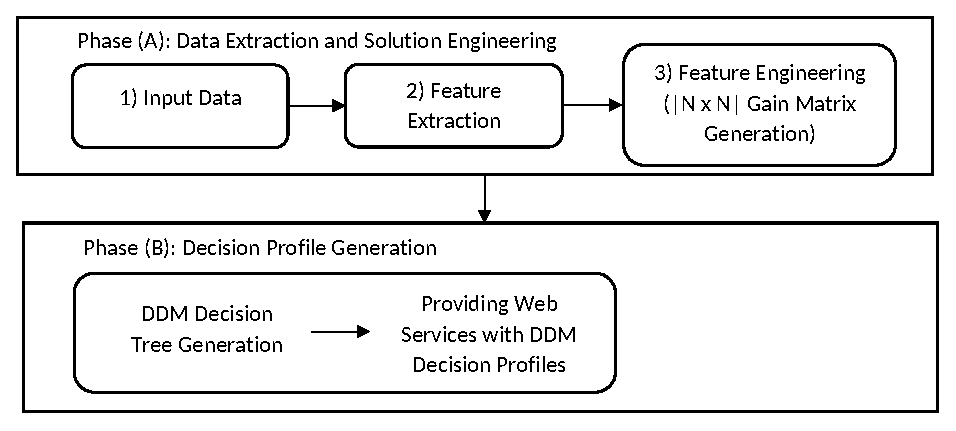
\includegraphics[width=5.25in]{figures/steps.eps}}
\caption{A summary of DDM decision profile generation steps}
\label{fig_steps}
\end{figure}

\subsection{Data Extraction and Solution Engineering}\label{ss:learningdata}

\subsubsection{Input Web Services Data}\label{sss:webservices}

%We used a data set extracted from running web services. In this data set,
Each web service is associated with a number of quality metrics that reflect its non functional parameters. These web services operate in an online environment and are continuously assigned tasks to handle. %To engage in communities, we add the external features that reflect web services' utility as a result of joining other web services to form a community (see Section \ref{s:ef}). %The additional features are %computed based on two assumptions that we adopt for a community to be formed.
We used the web services data set provided in \cite{10.1109/ISSRE.2011.17}. The raw data provides real-world QoS evaluation results from several users on 5,825 web services over 64 different time frames\footnote{http://www.wsdream.net/}. %In this data set, each web service is associated with a number of features that reflect its functionality.
%Our raw data set provides us with 64 different time slots of extracted features for each web service.
Using this data, we built a synthetic data set that contains features of a large number of web services and communities in different time intervals. The goal is to use the data set to train a decision-making model that adopts the trend of joining a community and use the model to predict/find the appropriate community for other web services. %To train our model, we build a decision tree as a benchmark for our decision making mechanism. The decision tree is made up by training the real data obtained from operating web services and extracting features related to their performance, either alone or as part of a joint effort with other web services. The ultimate objective is to propose for each web service and community the best joint decision about forming a group that maximizes every one's utility.

\subsubsection{Feature Extraction}\label{sss:filtereddata}

By processing the data provided for each web service over different time slots, we obtain the three internal quality features introduced in Section \ref{s:if}: \emph{throughput}, \emph{availability} and \emph{execution time} and the two external features discussed in Section \ref{s:ef}.  In fact, web services and communities are represented using feature vectors of these five internal and external features.

%To engage in communities, we add two additional external features that reflect web services estimation of its quality metrics compared to other web services.
%Therefore, we have generated an array of web services with three distinct features.

\begin{figure}%[!t]
\centerline{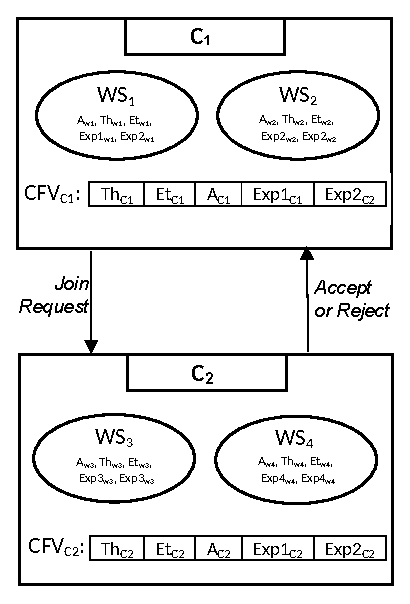
\includegraphics[width=3.15in]{figures/cfvs.eps}}
\caption{Communities with different properties of web services actively looking for other communities to collaborate with}
\label{fig_community}
\end{figure}

%By combining these three internal features to the two external features discussed in Section \ref{s:ef} that reflect the community's estimation of its quality metrics, we generate a set of feature vectors representing the communities of web services for training purposes.


We formulate a \emph{Community Feature Vector (CFV)} as $CFV_{<C>} = [f_1,...f_5]$ having a community of $k$ web services ($C = \{ws_1,...ws_k\}$, $k \geq 1$)\footnote{A web service is considered as a community of one web service.}. The features $f_1$ through $f_5$ represent the \emph{execution time}, \emph{throughput}, \emph{availability} and the \emph{external parameters 1 and 2} respectively. A set of communities, with their feature vectors and utilities evaluated, provides our algorithm with a raw training data set. We call this set of communities the \emph{template vector} $CS$, and the set of feature vectors associated with the \emph{template vector} is referred to as the \emph{community feature vector set (CFVS)}. Figure \ref{fig_community} depicts web services and communities looking to form new groups in order to improve their utility gain.

\subsubsection{Feature Engineering}\label{sss:feng}
Let $CFVS = \{CFV_{<C_1>}, \dots, CFV_{<C_N>}\}$ be the community feature vector set with $N$ communities. Based on the $CFVS$ set, we create an $|N \times N|$ gain matrix $gain^{t}$ for each time slot $t$. Each entry $gain_{n,m}^{t}$ corresponds to a utility gain of community $C_n$ when it joins community $C_m$. This gain is computed as follows: $gain_{n,m}^{t} = U_{C_n \cup C_m}^{t} - U_{C_{n}}^{t}$ where $U_{C_n \cup C_m}^{t}$ and $U_{C_{n}}^{t}$ are the utilities at time $t$ computed using Equation \ref{u_c_load}.  Evaluating the utility gain for all entries of the $gain^t$ matrix is a computationally heavy process when $N$, the size  of the feature vector set, is large. Therefore, this size should be chosen carefully.

\begin{table*}[ht]
\footnotesize
\caption{An example of $gain$ matrix for 3 different communities and their combinations} % title of Table
\centering % used for centering table
{\renewcommand{\arraystretch}{1.2}
\begin{tabular}{c|c c c c c c} % centered columns (4 columns)
\hline\hline %inserts double horizontal lines
 & \textless348\textgreater & \textless1934\textgreater & \textless2117\textgreater & \textless348, 1934\textgreater & \textless1934, 2117\textgreater & \textless348, 1934, 2117\textgreater \\ [0.5ex] % inserts table
%heading
\hline % inserts single horizontal line
\textless348\textgreater & - & 0.282708 & 1.027081 & 0.282708 & 18.027081 & 18.027081 \\
\textless1934\textgreater & -2.637483 & - & 6.969072 & -2.637483 & 5.509583 & 4.387725 \\
\textless2117\textgreater & 5.027081 & 2.969072 & - & 5.509583 & 2.969072 & 5.509583 \\
\textless348, 1934\textgreater & 0.0 & 0.0 & -3.851432 & - & -3.851432 & -3.851432 \\
\textless1934, 2117\textgreater & 2.969072 & 0.0 & 0.0 & 2.969072 & - & 2.969072 \\
\textless348, 1934, 2117\textgreater & 0.0 & 0.0 & 0.0 & 0.0 & 0.0 & - \\ [1ex] % [1ex] adds vertical space
\hline %inserts single line
\end{tabular}
}
\label{table:nonlin} % is used to refer this table in the text
\end{table*}

%Now, we let our set of communities in the $CFVS$ set, within $|T|$ time frame iterations, choose the the best communities to join.
Each community is provided with the corresponding row of data from the $gain^t$ matrix. Basically, $C_i$ is provided with the data in row $i$ of this matrix, which reports all the possible utility values $C_i$ can gain by joining different communities. By ordering the utility gain values of the row, each community is equipped with an ordered set of preferences over other communities it can join. We define $\geq_{i}^t$ as the preference order of community $i$ at time $t$.

Let $C_1 \geq_{i}^t C_2 \geq_{i}^t ~\dots~ C_{i-1} \geq_{i}^t C_{i+1} \geq_{i}^t ~\dots~ C_n$ be an ordered sequence of preferences for community $C_i$ at time $t$. Based on this sequence, we define $K^t(C_i, k)$ as a set of the $k$ most preferred communities of community $i$ at time $t$.
%\subsubsection{feature vector generation}\label{sss:fvg}
\begin{equation}\label{h_t_pref_top}
\begin{split}				
K^t(C_i, 0) = &\emptyset \\
K^t(C_i, k) = &\Big\{C_x | C_x \geq_{i}^t C_y ~\forall C_y \in CS ~\wedge~ C_x \neq C_y ~\wedge~ C_y \notin K^t(C_i, k-1) \Big\}				
\end{split}
\end{equation}
Based on $K^t(C_i, k)$, we define a set of communities $C_j$ for $C_i$ which are the $k$ most preferred communities for $C_i$ and $C_i$ belongs to the $k$ most preferred communities of $C_j$. This basically yields the preference in both sides.
\begin{equation}\label{l_t_top_both}
\begin{split}	
L^t(C_i,k) = \Big\{C_j | C_j \in K^t(C_i, k)~ \wedge~ C_i \in K^t(C_j, k)\Big\}
\end{split}
\end{equation}

Table \ref{table:nonlin} illustrates an example of a $gain$ matrix for 3 different communities and their combinations. Each row shows the gain the community can achieve by collaborating with other 5 communities. In this example, for community $\textless 348 \textgreater$ we have: \\
$K(\textless 348 \textgreater, 1) = \{\textless1934, 2117\textgreater\}$ and \\
$K(\textless 348 \textgreater, 2) = \{\textless1934, 2117\textgreater, \textless1934\textgreater\}$ \\
Since $\textless 348 \textgreater$ is the best preferred community of $\textless 1934, 2117 \textgreater$ and vice versa, therefore $L(\textless 348 \textgreater, 1)$ is not empty and contains the community $\textless1934, 2117\textgreater$.

Using the $gain$ matrix and the mentioned preference ordering relations, we are able to build a decision tree where the list of possible communities to join and their expected utilities are set.
% as well as the joined events that took place in different time slots.
In addition to the best choice, web services have access to other ordered choices and can look for the second best or third best if their first try is rejected by the target community. This aspect is analyzed in more detail in the following section, in which we launch experiments and investigate the effectiveness of the use of a decision tree with different decision layers in joining other communities and enhancing the overall utility.

\subsection{Decision Profile Generation}\label{ss:learningmodel}

Our goal is to create a decision making profile for each community in the
$CFVS$ set. We are creating an environment where the communities can experience the
outcomes of different strategies. The result will be a decision tree of the
feasible and utility-increasing moves over time. The root of the decision tree
represents a community in the $CFVS$ set, and the other nodes represent
the communities resulting from the parent node's action of joining them along with their feature values and
expected utility.


We let communities pick the best communities maximizing their utilities over different time frames. At time $t = 1$, we let each community in the $CFVS$ set choose the best community, which is a single community in the set $\{C_j\} = K^t(C_i, 1)$. If community $C_j$ also ranks $C_i$ to be the highest preferred community to join, meaning the set $L^t(C_i, k=1)$ is not empty, they would join each other. Having set $k = 1$ is a very strict and hardly satisfiable condition. In order to relax the requirement, we increase the value of $k$ by a rate $r$ proportional to time slot $t$: $k = 1 + |r \times t|$. On early steps of the training process, web services and communities are more strict, but as time goes on, we let them choose second and then third best options too. However, increasing $k$  increases the time complexity as well.

When communities $C_i$ and $C_j$ are in each other's top $k$ preference set, the new combined community, i.e., $C_i \cup C_j$ is added to the list of possible communities that can join others at time $t+1$. Moreover, for each community $C_i$ in our initial $CFVS$ set, we maintain a tree with the community $C_i$ as its root. Its children are all the communities that $C_i$ decided to join. As the scenario progresses over time, the merged communities may decide to join other communities. When communities $C_i$ and $C_j$ decide to join each other and create community $C_k$, the new community $C_k$ will be added as a child to both $C_i$ and $C_j$ nodes. At the end of the process, each community is utilized with a tree representing all possible combinations of communities it can join. Algorithm \ref{algo:dectree} illustrates the DDM tree creation procedure as pseudo-code.

\begin{algorithm}
\DontPrintSemicolon
\KwIn{$\langle r, gain^t_{n,n}, CFVS \rangle$ learning rate $r$, $|N \times N \times T|$ gain matrix, community feature vector}
\KwOut{A set of \emph{root} nodes of the decision trees}
$k \gets 1$\;
$nodes[N] \gets$ initialize $N$ tree nodes representing each community in CFVS\;
\For{$t \gets 1$ \textbf{to} $T$} {
	$k \gets 1 + round (r \times t)$\;
  \For{all $C_i \in CFVS$} {
	  \For{all $C_j \in L^t(C_i, k)$} {
      % The "l" before the If makes it so it does not expand to a second line
      \If{$C_i \in L^t(C_j, k)$}{
        $C_k \gets C_i \cup C_j$\;
				add $C_k$ to $CFVS$ set\;
				initiate $node_k$, representing $C_k$\;
				$nodes_i.addChild (node_k)$\;
				$nodes_j.addChild (node_k)$\;
      }
%      \Else{
%        $j \gets j + 1$\;
%      }			
		}
  }
%  $i \gets i + 1$\;
}
\Return{nodes}\;
\caption{{\sc DDM Decision Tree Algorithm}}
\label{algo:dectree}
\end{algorithm}

Having created $|n|$ trees, one per community, our communities are utilized with the different possible paths they can take to maximize their utilities. Using a distance function\footnote{See Section \ref{s:experiments} for an example of this function.}, communities and web services outside the training set can find the community that closely resembles their parameters within the $CFVS$ set. Those new communities can use the trees of the closest communities in the training set to have an estimation of the outcome of all possible joining actions they can take. By so doing, new communities can request to join the best communities which will maximize their gain. Such a request is most likely to be accepted as the decision considers the preferences and utility gain of the other side as well.

As a real scenario example from the used data set, Figure \ref{fig_tree} depicts a snapshot from a decision tree created by the DDM algorithm for a particular singleton community $C_{1273}$. This tree shows the different communities that $C_{1273}$ has experienced with during the training process. Each line shows the web services list within a community, the community's feature vector and the last value on each line is the overall gained  utility of the community.


\begin{figure}%[!t]
\centerline{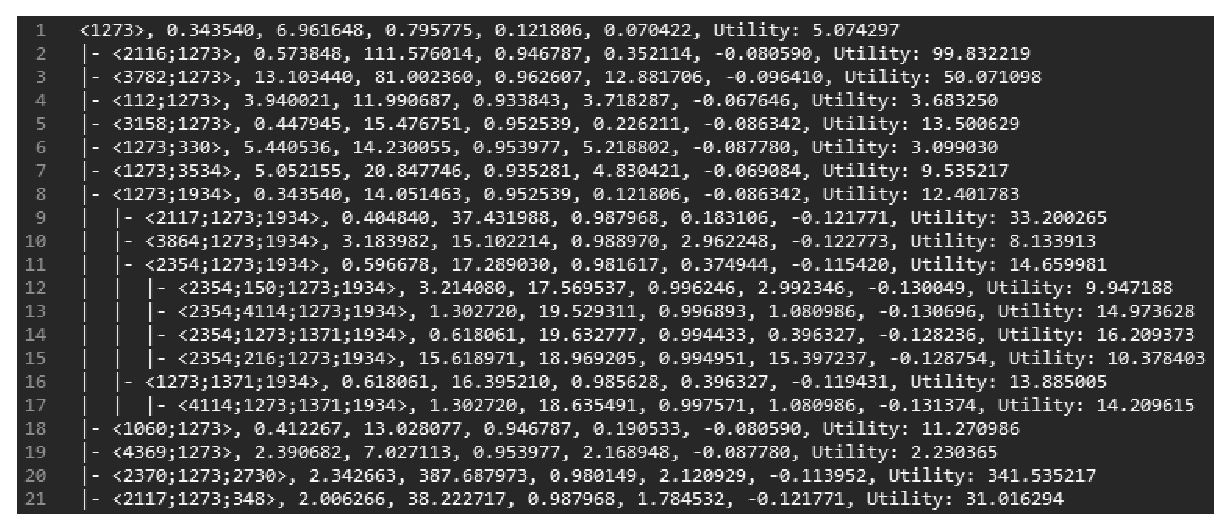
\includegraphics[width=6.25in]{figures/tree1.eps}}
\caption{A partial view of a decision tree created by DDM}
\label{fig_tree}
\end{figure}

\textbf{Complexity.} Here we analyze the computational complexity of the DDM decision tree creation algorithm on each time iteration $t$. Computing top $k$ preferred communities for $C_i$ in $K^t(C_i, k)$ requires $O(n.log(n))$ sort time. The size of $K^t(C_i, k)$ is $k$, and for each of those $k$ communities, we need to check against their $k$ top preferred communities, which needs $O(k^2)$. Line 5 iterates through $n$ communities, Line 6 takes $O(n.log(n))$ to compute and iterates $k$ times, and considering we already have the list sorted, Line 7 can reuse the sorted preferences. Thus, Line 7 takes $O(k)$ time to check if $C_i$ is member of $K^t(C_i, k)$. Multiplying these iterations, the order of complexity of the algorithm with regard to $n$ and $k$ for each time slot is: $O(k^2 \times n^2.log(n))$. Since the whole algorithm runs $T$ times, the overall complexity is $O(T \times k^2 \times n^2.log(n))$.

\section{Experiments}\label{s:experiments}
We implemented DDM in Java\footnote{Source code of implementation and data is available at: $https://github.com/Marooned202/DDM$}. We recall that we have extracted the set of features for 4532 web services in 64 different time slots through a data set provided in \cite{10.1109/ISSRE.2011.17}. By randomly choosing 86 web services out of this data set for each run, and selecting a subset of all possible combinations of sizes 2, 3, and 4 of these 86 web services, we have been able to create 10,000 communities and evaluated the feature vectors and utilities they can have in the 64 time slots. This provides us with the initial training feature set of size $|CFVS| = 10,000$ communities. Based on Equation \ref{u_c_load}, the utilities of these communities are estimated, and then the $gain$ matrix of size $|10,000 \times~ 10,000|$ of all possible ways of merging these 10,000 communities is generated\footnote {The template vector and $gain$ matrix generated are available at $https://github.com/Marooned202/DDM/tree/master/wsds/data/run$}. Based on the $gain$ matrix, each community has an ordered preference among other communities in the set.

We let communities and web services adopt their strategies based on our $DDM$ decision making mechanism. Based on the decisions adopted, each community will generate a decision tree profile. We let DDM run four times with different $r$ rates of 0.05, 0.07, 0.10 and 0.20. With the slow rate of $r = 0.05$, we increase $k$ in Equation \ref{u_c_normal} for every 20 time frames, which will happen only three times in our 64-step experiment. In the case of $r = 0.20$, $k$ increases much faster, at a rate of once every 5 time frames, which increases the complexity of the $L^t(C_i,k)$ search for each community in the $CFVS$ set.

Table \ref{table:valueandgain} depicts the average utility gain value of the communities in each of the four runs. The utility gain is the increase of utility the communities gain by cooperating and joining other communities. The utility gain ratio is the ratio of their final utility over initial utility. Comparing the different search rates, we can see that increasing the value of $r$ from $0.05$ to $0.10$ results in a significant performance boost. However, higher rates of $r$ ($r > 0.10$) are not increasing the chance of finding better collaborative groups for our communities while unnecessarily increasing the search complexity.

\begin{table}[ht]
\caption{Utility gain of web services after making collaborative groups based on DDM algorithm with different $r$ rates} % title of Table
\centering % used for centering table
{\renewcommand{\arraystretch}{1.2}
\begin{tabular}{c|c|c} % centered columns (4 columns)
\hline\hline %inserts double horizontal lines
Search Rate $r$ & Utility Gain Value & Utility Gain Ratio \\ [0.5ex] % inserts table
%heading
\hline % inserts single horizontal line
r=0.20 & 176.1499 & 6.9690 \\
r=0.10 & 174.6541 & 6.9182 \\
r=0.07 & 159.9462 & 6.2834 \\
r=0.05 & 136.0768 & 5.1032 \\ [1ex] % [1ex] adds vertical space
\hline %inserts single line
\end{tabular}
}
\label{table:valueandgain} % is used to refer this table in the text
\end{table}


%\begin{figure}%[!t]
%\centering
%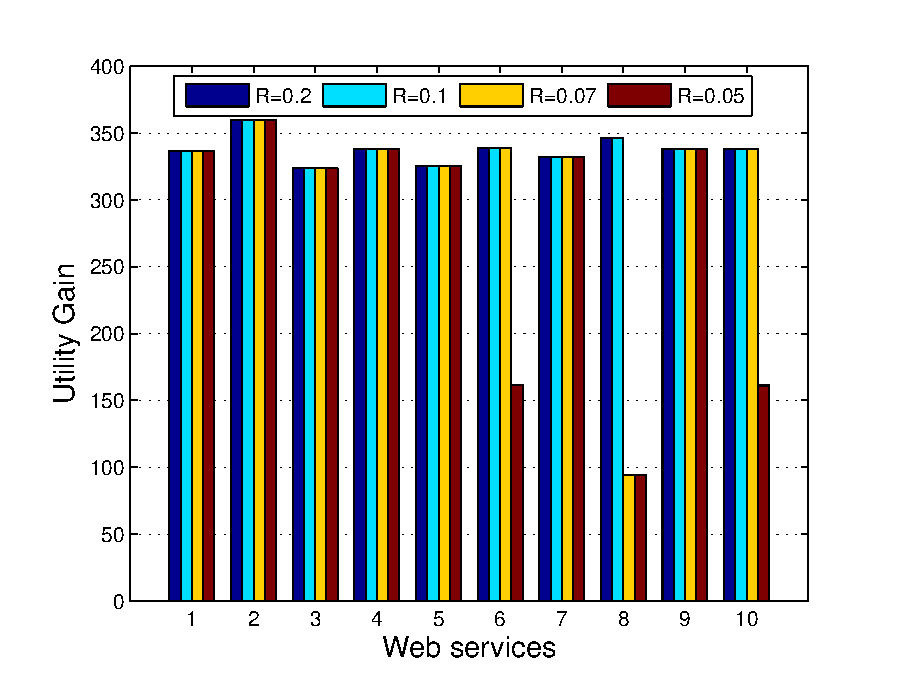
\includegraphics[width=3.5in]{figures/utility_gain_r.eps}
%\caption{DDM Utility Gain Value}
%\label{utility_gain_value}
%\end{figure}
%
%\begin{figure}%[!t]
%\centering
%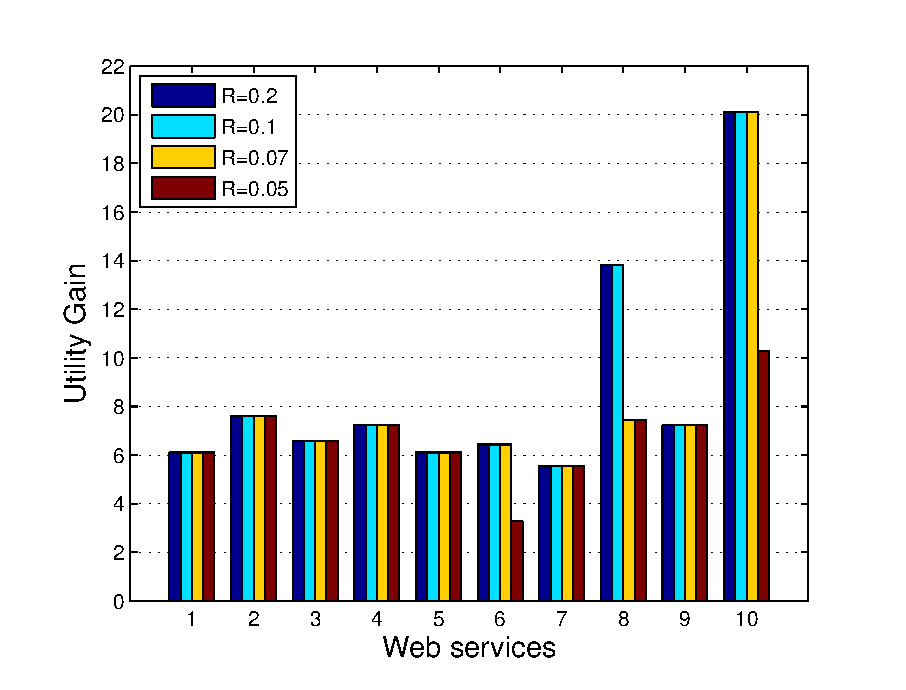
\includegraphics[width=3.5in]{figures/utility_ratio_r.eps}
%\caption{DDM Utility Gain Ratio}
%\label{utility_gain_ratio}
%\end{figure}


The closest related work \cite{10.1109/TSC.2012.12,
DBLP:conf/IEEEscc/LimTMB12, DBLP:conf/IEEEscc/KhosravifarABT11} and our
previous work \cite{journal-community-formation} regarding the community formation problem have considered a centralized approach where a community manager has complete information of all the web services and their quality
metric and parameters. Those proposals run complex algorithms through all the space of
solutions in order to find the optimal answer. However, in this research work, we
have considered an unexplored and more realistic situation where information is incomplete and a decision
profile is generated based on a smaller set of web services. Our solution helps
communities and web services select actions that lead towards
maximizing their utilities. Therefore, considering the different settings,
we cannot experimentally compare our work with the mentioned related work.


To compare our work against a benchmark, we utilize the same communities and web services with a simple rational decision making mechanism in which a community will choose to join another one if it increases its utility by any amount, without aiming to be optimal. We call this method the {\textit{rational} method. We have chosen 10 random web services and compared the results with web services which adopted our DDM model. Figure \ref{utility_gain_mlisa_and_rational} shows the comparison of the end result of utility gain values. In 18 out of 40 tries, \emph{rational} agents were not able to improve their utility at all because the communities they chose rejected their request, most likely because they would not have increased the utility of the other communities if they had joined them. The results show that a long-term strategic decision mechanism is needed to satisfy all the services within communities. Figure \ref{utility_gain_mlisa_and_rational_ratio} shows the same results in terms of ratio of utility gain.

\begin{figure}%[!t]
\centering
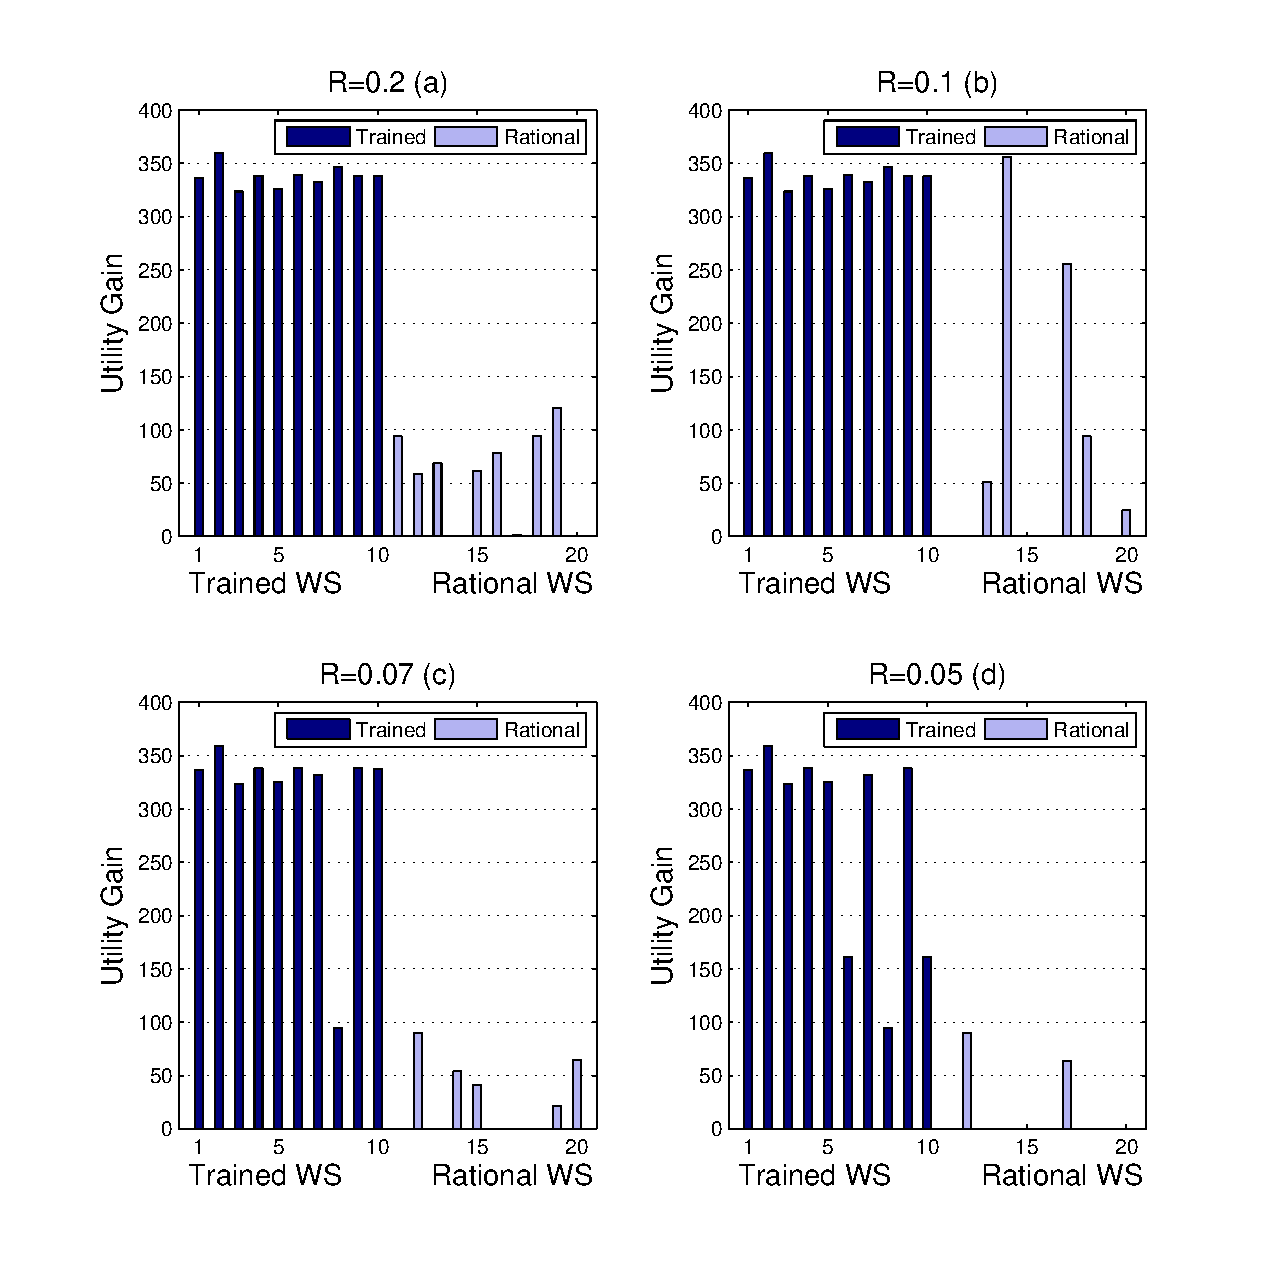
\includegraphics[width=3.5in]{figures/utility_gain.eps}
\caption{DDM against Rational: utility gain }
\label{utility_gain_mlisa_and_rational}
\end{figure}

\begin{figure}%[!t]
\centering
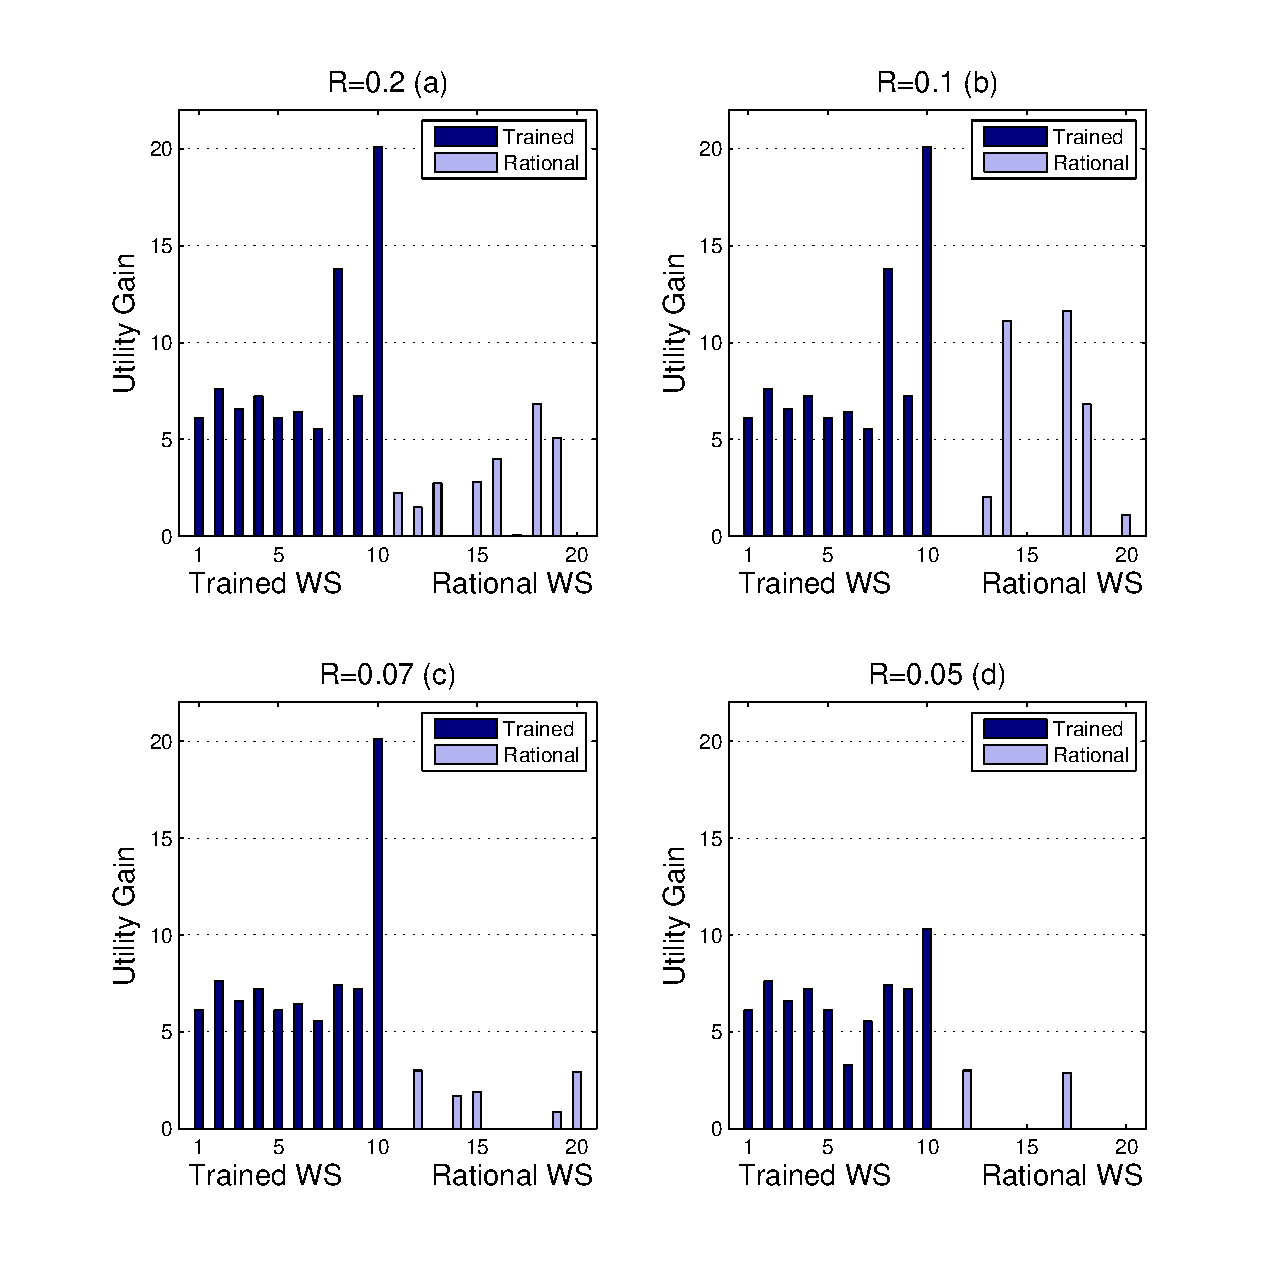
\includegraphics[width=3.5in]{figures/utility_ratio.eps}
\caption{DDM against Rational: ratio of utility gain}
\label{utility_gain_mlisa_and_rational_ratio}
\end{figure}

Now, we evaluate the performance of the decision profiles generated based on our data set for other communities.% which are not included in the decision tree creation process.
We create 1,000 communities from the web services in the data set that were not involved in the training process of our decision model. We define a distance function that measures the difference between basic features of communities, which measures the similarity among communities.

\begin{equation}\label{distance_c}
\begin{split}
distance (C_1, C_2) & = |Th_{C_1} - Th_{C_2}| \\
                    & + |A_{C_1} - A_{C_2}| + |Et_{C_1} - Et_{C_2}|
\end{split}
\end{equation}

Now, each community tries to find the closest community within the trained $CFVS$ set. Following its decision profile, the community can get a good estimate of the possible strategic decisions it can adopt. Basically, the trained profiles benefit the new communities in two ways. First, they provide the communities with a set of viable communities to join. Second, they provide an estimation of long-term utility gain for each available decision. In this experiment, we let communities follow the best decision within the decision tree provided to them.


In order to evaluate the performance of the mechanism, we used \emph{Receiver Operating Characteristic (ROC) curve}, which is a graphical plot illustrating the true negative rate against the false positive rate at various threshold settings in classifier systems. In order to classify our communities' selection strategies correctly, for each community, we evaluated the training process by replacing the community in the set with the closest one, from which it gets the strategy profile. If the actions are the same and the same utility levels are gained, we classify the decision as correct. Otherwise, it is classified as a wrong decision. \emph{AUC}, the area under the \emph{ROC curve}, is equal to the probability that a classifier will rank a randomly chosen positive instance higher than a randomly chosen negative one, and the higher the number the better the solution, which reflects better performance.  Figure \ref{roc5} illustrates the \emph{ROC curve} evaluation of the DDM decision making mechanism. As benchmark, we compare our method with two other methods: the \emph{rational} method and the \emph{greedy} method. The \emph{greedy} method only looks up the available list of communities and simply joins the community that maximizes its utility without considering any long-term strategy or other communities' acceptance scenarios. It is a greedy algorithm that focuses on choosing a locally optimal choice.

\begin{itemize}
  \item {\bf Rational Method:} Communities would send a join request to any available community, which will increase the utility. The other community would accept the join offer if its own utility gain is positive as well.
	\item {\bf Greedy Method:} Communities do a linear search among all the available communities and send a join request to the community which results in maximum utility. The other community would accept the join offer if its own utility gain is positive and the utility gain does not need to be the maximum for the community receiving the join request.
\end{itemize}

Figure \ref{roc5} compares the results for all the methods. The \emph{rational} and \emph{greedy} methods have very high failure rates compared to our method. Table \ref{fail_rate} illustrates the number of communities that failed to find the optimal collaboration group. The results support the need for a long-term training model in a successful decision making process.

\begin{figure}%[!t]
\centering
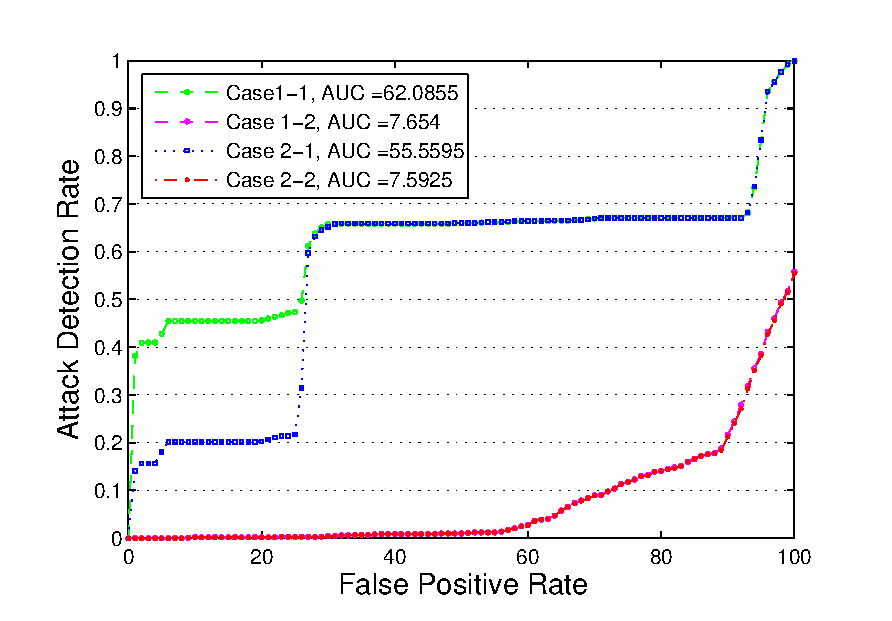
\includegraphics[width=3.5in]{figures/roc.eps}
\caption{RoC Curve}
\label{roc5}
\end{figure}

\begin{table}[ht]
\caption{Number of communities that misses the optimal decision, out of 1,000 communities} % title of Table
\centering % used for centering table
\begin{tabular}{|c|c|} % centered columns (4 columns)
\hline %inserts double horizontal lines
 Method&Miss \\ [0.5ex] % inserts table
%heading
\hline % inserts single horizontal line
 DDM r=0.05& 375 \\ % inserting body of the table
 DDM r=0.07& 137 \\
 DDM r=0.10& 6 \\
 DDM r=0.20& 6 \\
Rational Method& 717 \\
Greedy Method& 828 \\ [1ex] % [1ex] adds vertical space
\hline %inserts single line
\end{tabular}
\label{fail_rate} % is used to refer this table in the text
\end{table}


Now, we evaluate the system-specific results from users' and communities' perspectives. By distributing tasks among the communities over the 64 time frames, we evaluate the revenue for each community. Figure \ref{stats1} shows the overall revenue gain of communities using our method. Figure \ref{stats2} shows the momentarily revenue gain for each community in each time slot compared to the previous time. These results show that the run with the higher learning rate of $r=0.20$ starts discovering better communities to join much earlier. The runs with slow rates seem to find some communities to join initially, but then they slow down until later, when they start discovering new communities to join.


\begin{figure}%[!t]
\centering
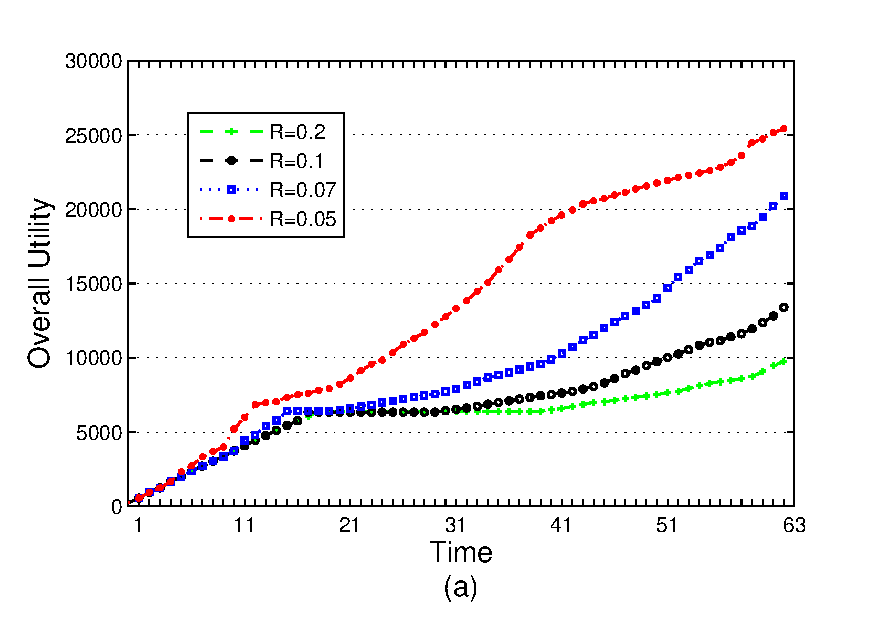
\includegraphics[width=3.5in]{figures/stats1.eps}
\caption{Overall utility of all the communities}
\label{stats1}
\end{figure}


\begin{figure}%[!t]
\centering
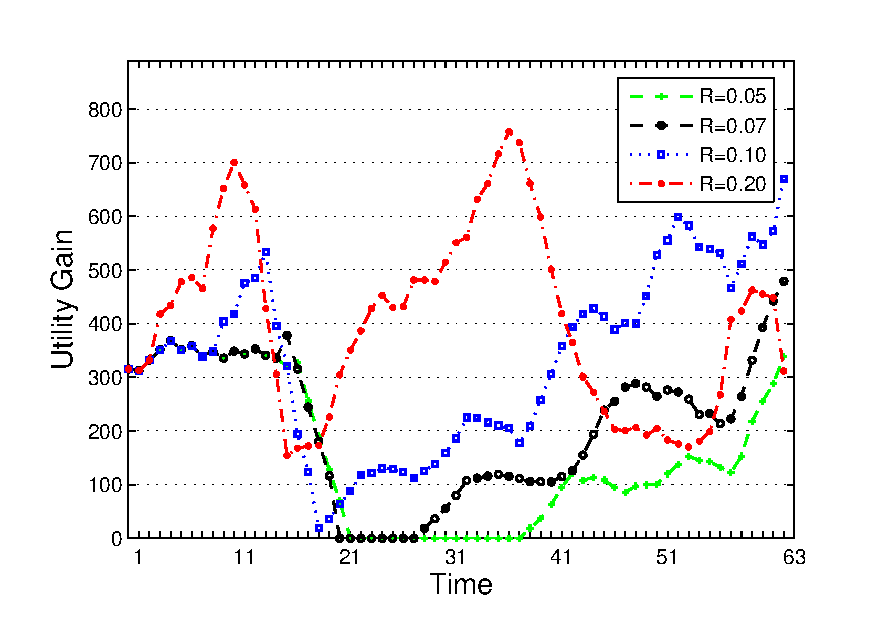
\includegraphics[width=3.5in]{figures/stats2.eps}
\caption{Utility gain over time}
\label{stats2}
\end{figure}

Figure \ref{stats3} depicts the average community size over time, which essentially represents the number of new communities being formed. The results show once again the communities using DDM with higher search rates grow faster in size, implying that the communities find appropriate web services to join with faster.

\begin{figure}%[!t]
\centering
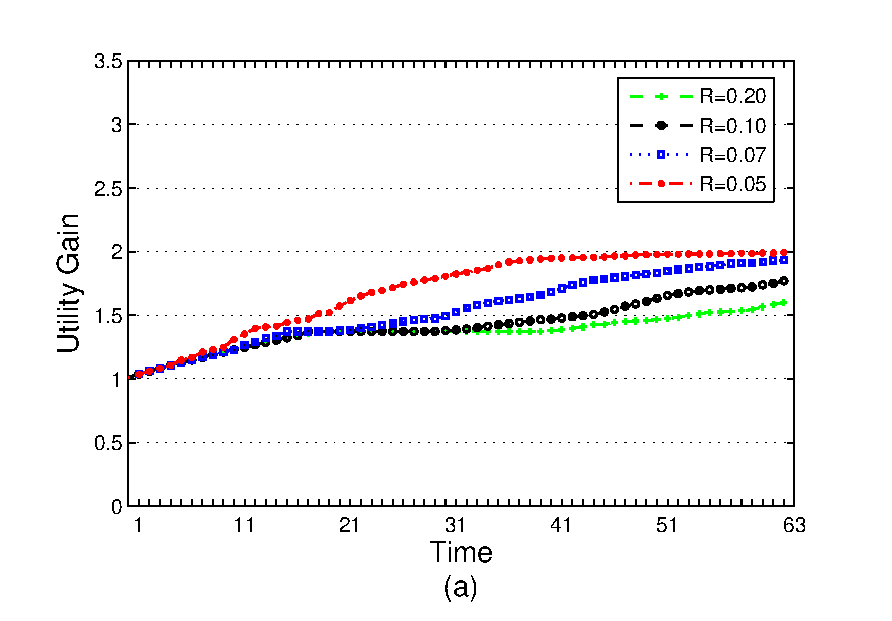
\includegraphics[width=3.5in]{figures/stats3.eps}
\caption{Average community size}
\label{stats3}
\end{figure}



\section{Related Work}\label{s:related_work}

Most of the recent work on communities of services are either
user-centric and focus on user satisfaction
\cite{Chun02user-centricperformance} or system-centric and focus
on the whole system throughput, performance and utilization. There
are many contributions in distributed, grid, cluster and cloud
services which are system-centric. However, in real world
environments and applications, both users and service providers
are self-interested agents, aiming to maximize their own profit.
In those environments, both parties (users and services) will
collaborate as long as they are getting more benefits and payoff.

In this direction, recently \cite{DBLP:conf/IEEEscc/LimTMB12,
DBLP:conf/IEEEscc/KhosravifarABT11, 10.1109/TSC.2012.12} proposed
mechanisms to help users and services maximize their gain. A
two-player non-cooperative game between web services and community
master was introduced in
\cite{DBLP:conf/IEEEscc/KhosravifarABT11}. In this game-theoretic
model, the strategies available to a web service when facing a new
community are requesting to join the community, accepting the
master's invitation to join the community, or refusing the
invitation to join. The set of strategies for communities are
inviting the web service or refusing the web service's join
request. Based on their capacity, market share and reputation, the
two players have different sets of utilities over the strategy
profiles of the game. The main limits of this game model are: 1)
its consideration of only three quality parameters, while the
other factors are simply ignored; and 2) the non-consideration of
the web services already residing within the community. The game
is only between the community master and the new web service, and
the inputs from all the other members and their influence on the
master's decision are simply ignored. The consideration of those
inputs and this influence factor is a significant issue as
existing web services can lose utility or payoff because of the
new member, which can result in an unhealthy and unstable group.
The problem comes from the fact that the existing members should
collaborate with the new web services, so probably their
performance as a group can suffer. Existing members may even
deviate and try to join other communities if they are unsatisfied.
Those considerations of forming stable and efficient coalitions
are the main contributions of our thesis.

In \cite{DBLP:conf/IEEEscc/LimTMB12}, a 3-way satisfaction approach
for selecting web services has been proposed. In this approach,
the authors proposed a web service selection process that the
community masters can use. The approach considers the efficiency
of all the three involved parties, namely users, web services and
communities. In this work, it is shown how the gains of these
parties are coupled together using a linear optimization process.
However, the optimization problem in this solution tends to
optimize some parameters considering all web services regardless
of their efficiency and contribution to the community's welfare.
Moreover, there are no clear thresholds for accepting or rejecting
new web services. The solution of the optimization problem could,
for instance, suggest web services already residing within the
community to increase or decrease their capacity to cover up the
weakness of other parties in the system. However, a high
performing web service could deviate anytime it finds itself
unsatisfied within the community instead of adjusting its service
parameters.

In \cite{10.1109/TSC.2012.12}, a cooperative scheme among
autonomous web services based on coalition game theory has been
introduced. The authors have proposed an interesting algorithm to
reach individually stable coalition partition for web services in
order to maximize their efficiency. The communities choose new web
services on the promise that it would benefit the community
without decreasing any other web service's income. In the proposed
model, the worth of community is evaluated with high emphasis on
the availability metric and considering price and cost values
only. The community structure is based on a coordination chain,
where a web service is considered as a \emph{primary} web service
and the community task-distribution method initially invokes the
primary web service and only if the primary web service is
unavailable, the method invokes the next backup web services as
they are ordered in the coordination chain. We believe that this
coordination chain limits the cooperation power as it introduces a
sort of hierarchy. However, in pure and open cooperative models,
such as the one we propose in this paper, active cooperation
activities engaging simultaneously many agents so that they can
perform the tasks more efficiently are being used. Moreover, if
the availability is high, which is the case nowadays with the
recent advancements in cloud infrastructures and hardware technologies, the
backup web services will end-up having a very low chance of
getting jobs, especially the ones further in the chain. This will
results in a considerable waste of web services capabilities.

All the proposed frameworks share a common aspect, which is providing the solution based on assumption of having complete information of all services and performing evaluations based on a large number of input each time they want to adopt a strategic decision making process.
So basically, these solutions generally suffer from high complexity, which makes decision making very hard, even impossible in some cases in a real-time fashion, or they simplify important aspects to make it practical in the real world, thereby hurting the decision making performance. We address this issue by introducing DDM a framework that operates based on a trained model that regulates web service agents' decision making process in terms of cooperating with one another. After being trained, web services get to compute expectations as utilities they would gain while cooperating with communities of different characteristics. Therefore, web services and communities can make prudent decisions when inviting a web service to join or accepting a join inquiry initiated from a web service. In general, DDM equips web services with efficient methods for foreseeing how their choices will impact their long-term and short-term goals; therefore, opting for best decision available. \\

\noindent \textbf{Web Service Communities}

Here we introduce the related research work regarding the engineering and formation of communities of web services. In \cite{DBLP:journals/internet/BenatallahSD03}, Benatallah et al. defined communities of web services as \emph{Service Containers} that aggregate substitutable web services having the same set of operations and providing common functionalities. They abstracted \emph{Service Containers} as web services that are created, advertised, discovered and invoked just as elementary web services. The \emph{Container} is considered as a manager that is responsible for web service selection upon receiving a request on run-time. The authors have proposed a scoring technique based on non-functional requirements of the request and web service capabilities to dynamically chose the web service to perform the requested task. A similar concept was proposed by Maamar et al. in \cite{DBLP:journals/ijebr/MaamarSTBB09}. The authors introduced web service communities as a collection of web services with a common functionality but different QoS properties. A community manager, upon receiving a request, delegates the request to one of its current members. The choice is based on the performance history and quality metrics of each web service. The authors have proposed an efficient global web service selection algorithm in order to approach quality constraints and preferences for composite services which requires aggregation of different types of services to satisfy the user. In the same line of research, Benslimane et al. \cite{Liris-2770} have proposed a multi-layer approach grouping similar web services into communities and having an interface implemented as an abstract web service for accessing the community. The considered layers are: composite, management and community. The interactions among those layers and the bindings are performed by a generic driver called Open Software Connectivity (OSC). However, unlike our work, these proposals only tackle the problem of internal community management from the task execution perspective, but not the problem of community formation and the one of dynamically selecting which community to join and which web service to invite. Moreover, the web services selection process is done centrally by the community manager, while we address the problem more realistically from the distributed angle.

In \cite{managing-hela-jalel}, Limam and Akaichi have proposed web
service communities with centralized access across distributed web
services. They have proposed a framework for web service
management, query resolution among communities and a query caching
mechanism executed by the manager to improve the performance of
query resolution process among many distributed communities. The
key idea is to cache previous computed results for answering
future queries. Maamar et al. initially in \cite{conf/webist/MaamarLBTS07} and
then comprehensively in \cite{DBLP:journals/ijebr/MaamarSTBB09}
proposed an architecture utilizing \emph{Contract-Net} protocol
for engineering task distribution within communities of web
services. The protocol is centrally executed by the community
manager. This architecture has been further extended in
\cite{CSTintercommunity, conf/IEEEscc/BenharrefSBB11,
conf/IEEEscc/KhosravifarBMMT10, conf/aina/LimTM11}. Two types of
roles have been distinguished for community members: masters and
slaves. Master web services are community managers that lead
communities and are responsible for membership management. They
can invite and convince slave web services to join the community,
and attract new slave web services to their communities by
awarding them better payoff. Moreover, they can eject some slave
members from the community to improve its overall reputation if
these members are misbehaving or cannot provide the promised QoS.
In \cite{Medjahed05adynamic}, Medjahed and Bouguettaya have
developed a community as a ``cluster'' that groups Web services
based on a specific area of interest. All web services in a given
community share the same functionality. These communities are
created by \emph{third party community providers} which use the
\emph{community ontology} as a template and define a set of
operations that all web services within a community should
provide. Using semantic analysis on web service operations, web
services either find and join a community with similar
functionality or create a new operation description for a new
community. The authors have described the concept of
\emph{community agents} associated to \emph{community providers}.
A community agent is responsible, among other things, of the
registration of services with the community. An example of a
community that provides health care services to senior citizens
has been used. In this example, a governmental entity is needed to
check the health care standards used by the members before
authorizing them to be part of the community. Such a central
entity is represented by the community agent. Thus, community
agents are playing the role of community managers. In a close work
\cite{Zeng:2003:QDW:775152.775211}, Zeng et al. have described a
global planning selection algorithm and a delegation algorithm to
be run when a request to execute an operation is received by the
community. This needs a central entity to run those algorithms.
Such entity plays the same role as the community coordinator or
manager. All these proposals have in common the consideration
of the central entity for community management, which includes the hiring and firing of the community members, while our approach is fully distributed. Moreover, the stability of the community has not been investigated. Another major difference with our work is that the decision making process is only one way and unilateral from the community manager perspective. In our contribution, both participants, namely communities and web services, participate in the decision making process and a joining decision is made only if it is the best option for both players.


%%%%%%%%%%%%%%%%%%%%%%%%%%%%%%%%%%%%%%%%%%%%%%%%%%%%%%%%%%%%%%%
\section{Summary}\label{sec:conclusion-cha4}

In this research work, we proposed a training model for the problem of membership management of communities of web services. Using the traning model we created a decision making profile for each community and web service involved which provides them with a set of feasible and utility increasing moves. This utilized our web services with efficient methods of foreseeing how their choices of actions would impact their long-term and short-term goals, therefore they opted for best decision available. The ultimate goal is to choose the best decision when it comes to communities formation, among many possible short-term rational and utility increasing choices. The experimental results show that our algorithms provide web services and community owners, in real-world-like environments, with applicable and near-perfect decision making mechanisms. The results of experiments using real data samples support the need for a long-term training model in a successful decision making process.

Our plan for future work is to advance learning process on the training set that we provided in our work. SVN machine learning algorithm are suitable in classification of our training data set, to better classify correct or wrong decisions based on long-term utility gains, as data set outputs. This can further facilitate the process of finding optimal cooperators in regards to enhancing web services' overall performance as service providers.

In next chapter, we analyse the internal community behaviour of web services, and propose a model for competing and cooperating agents within the communities of web services.
